\documentclass[conference]{IEEEtran}
\IEEEoverridecommandlockouts

\usepackage{cite}
\usepackage{amsmath,amssymb,amsfonts}
\usepackage{algorithmic}
\usepackage{graphicx}
\usepackage{textcomp}
\usepackage{xcolor}
\usepackage[T1]{fontenc}
\usepackage[utf8]{inputenc}
\usepackage[spanish,es-noquoting]{babel}
\usepackage{hyperref}
\hypersetup{
    colorlinks=true,
    linkcolor=black,
    citecolor=black,
    urlcolor=blue
}
\usepackage{listings}
\usepackage{tikz}
\usetikzlibrary{shapes,arrows,positioning,babel}

\lstset{
  language=C++,
  basicstyle=\ttfamily\scriptsize,
  keywordstyle=\color{blue}\bfseries,
  stringstyle=\color{red},
  commentstyle=\color{green!60!black},
  numbers=left,
  numberstyle=\tiny\color{gray},
  stepnumber=1,
  numbersep=4pt,
  xleftmargin=1.8em,
  framexleftmargin=1.5em,
  frame=single,
  framesep=3pt,
  aboveskip=7pt,
  belowskip=7pt,
  breaklines=true
}
\renewcommand{\lstlistingname}{Código}

\makeatletter
\def\lst@makecaption#1#2{%
  \vskip 5pt
  \centerline{\normalfont\footnotesize\bfseries #1: \mdseries #2}%
  \vskip 7pt
}
\makeatother

\begin{document}

\title{Especificación Formal en VDM++ y Verificación de Márgenes Temporales de Cierre (UPPAAL) para Control Preventivo de Compuertas en Redes de Riego\\
}

\author{\IEEEauthorblockN{Marco Ramiro Quispe Flores}
\IEEEauthorblockA{\textit{Escuela Profesional de Ingeniería de Sistemas} \\
\textit{Universidad Nacional de San Agustín de Arequipa}\\
Arequipa, Perú \\
mquispeflores@unsa.edu.pe}
\and
\IEEEauthorblockN{Francis Willian Ayamamani Anasco}
\IEEEauthorblockA{\textit{Escuela Profesional de Ingeniería de Sistemas} \\
\textit{Universidad Nacional de San Agustín de Arequipa}\\
Arequipa, Perú \\
fayamamani@unsa.edu.pe}
\and
\IEEEauthorblockN{William Herderson Choquehuanca Berna}
\IEEEauthorblockA{\textit{Escuela Profesional de Ingeniería de Sistemas} \\
\textit{Universidad Nacional de San Agustín de Arequipa}\\
Arequipa, Perú \\
wchoquehuancab@unsa.edu.pe}
\and
\IEEEauthorblockN{Brayan Denilson Choquehuanca Bedoya}
\IEEEauthorblockA{\textit{Escuela Profesional de Ingeniería de Sistemas} \\
\textit{Universidad Nacional de San Agustín de Arequipa}\\
Arequipa, Perú \\
bchoquehuancab@unsa.edu.pe}
}

\maketitle

\begin{abstract}
En las redes de distribución de agua para agricultura, las crecidas intempestivas de caudal representan un riesgo crítico cuando los retardos de muestreo y de cierre electromecánico de compuertas superan el margen de borde libre del canal. A diferencia de los sistemas SCADA tradicionales con controladores lógicos programables (PLCs) basados en heurísticas empíricas que asumen respuesta instantánea, este artículo presenta un marco formal dual orientado a verificar la lógica de control y determinar matemáticamente su margen seguro de reacción temporal (\textit{Worst-Case Reaction Time}, WCRT). En la primera fase, se especifica en VDM++ una arquitectura orientada a objetos de cinco clases (\texttt{Sensor}, \texttt{Compuerta}, \texttt{Canal}, \texttt{Controlador} y \texttt{Test}) que integra regulación preventiva en tres niveles (\texttt{<NORMAL>}, \texttt{<PRECAUCION>} con apertura parcial al 50\% y \texttt{<CRITICO>} con cierre y alivio), balance volumétrico efectivo e historial secuencial de telemetría; la especificación se valida sin errores de sintaxis ni tipos en Overture Tool v3.0.2, ejecutando la suite \texttt{Test.vdmpp} con un 100\% de cobertura en las cinco clases del modelo. En la segunda fase, se modela en UPPAAL 5.0 una red de cuatro autómatas temporizados con acoplamiento físico estricto (\texttt{Controlador} $\rightarrow$ \texttt{Compuerta} $\rightarrow$ \texttt{MedioAmbiente}), retardo mecánico explícito de cierre ($T_{\text{cierre}}$) e histéresis anti-\textit{chattering} ($[60, 80]\,\text{m}^3$). Mediante lógica temporal CTL, se demuestra un contraejemplo formal de desborde ($105 > 100\,\text{m}^3$) cuando $T_{\text{cierre}} \geq 9\,\text{s}$, se establece la frontera matemática segura $T_{\text{cierre}} \leq 8\,\text{s}$ y se certifican siete propiedades críticas de ausencia de bloqueos ($A[] \text{ not deadlock}$), contención ($A[] \text{ volumen} \leq 100$), vivacidad y recuperación por histéresis para $T_{\text{cierre}} = 6\,\text{s}$ (pico de $95\,\text{m}^3$).
\end{abstract}

\begin{IEEEkeywords}
Métodos Formales, VDM++, Model Checking, UPPAAL, Worst-Case Reaction Time, Histéresis, Canales de Riego, SCADA.
\end{IEEEkeywords}

\section{Introducción}
La seguridad hídrica en la agricultura de regadío constituye un eje estratégico para el desarrollo económico y la sostenibilidad de las cuencas áridas y semiáridas. En el Perú, diagnósticos oficiales de la Autoridad Nacional del Agua y el Banco Mundial revelan que más del 80\% de la infraestructura de riego en cabeceras de cuenca carece de instrumentación y automatización, lo que ocasiona pérdidas de conducción superiores al 45\% y una alta vulnerabilidad ante crecidas intempestivas \cite{bancomundial2016seguridad}. En la región de Arequipa, infraestructuras de envergadura como el Proyecto de Irrigación Majes Siguas I sufren de desbalances recurrentes derivados de la manipulación manual y tardía de compuertas de derivación ante variaciones imprevistas del caudal matriz \cite{zapana2018respuestas}. Estudios recientes en redes hidráulicas demuestran que las compuertas analógicas operadas sin coordinación automática presentan eficiencias inferiores al 52\%, donde los picos de sobreflujo dañan los terraplenes por ausencia de cierre preventivo \cite{dominguez2024impacto}.

Desde la perspectiva del control automático, los canales abiertos presentan dinámicas no lineales complejas, retardos de transporte variables y una interacción hidrodinámica acoplada entre tramos sucesivos \cite{hernandez2020control}. El Manual 131 de la Sociedad Americana de Ingenieros Civiles (ASCE) estipula márgenes estrictos de resguardo libre (\textit{freeboard}) y exige tiempos de reacción acotados en compuertas para impedir el rebase de bordos \cite{wahlin2016canal}. No obstante, la automatización industrial convencional (SCADA/PLC) implementa lógicas de control programadas empíricamente que, frente a retardos electromecánicos, oscilaciones rápidas (\textit{chattering}) o eventos límite, generan anomalías de temporización y accidentes operativos \cite{gleirscher2020formal}.

Para superar estas limitaciones, la ingeniería de software crítico recurre a los \textit{métodos formales} \cite{woodcock2009formal,clarke1996formal}. A diferencia de las pruebas de software convencionales que solo muestrean un conjunto finito de trayectorias, la verificación formal provee demostraciones matemáticas de que el sistema satisface sus requerimientos en la totalidad del espacio de estados \cite{sinha2019survey}.

El aporte diferencial del presente trabajo frente a un sistema SCADA convencional radica en pasar de un esquema reactivo \textit{On-Off} supuesto instantáneo a un marco formal en dos etapas antes de la síntesis en PLC: primero, la especificación orientada a objetos en VDM++ \cite{larsen2010vdmmanual} de un controlador SCADA desacoplado del medio físico \cite{fitzgerald2010collaborative}, con control preventivo por etapas, balance volumétrico e integridad sobre conjuntos, secuencias y mapas \cite{bowen1994seven}; y segundo, la verificación temporizada en UPPAAL \cite{behrmann2004tutorial,bengtsson2004timed} que incorpora el retardo físico de cierre de la compuerta y la histéresis para demostrar mediante contraejemplo cuándo falla el sistema y certificar la cota temporal máxima segura de operación.

\section{Trabajos Relacionados}
La aplicación de técnicas de automatización y verificación en redes hídricas ha sido abordada desde diversos enfoques en la literatura científica:

\textit{1) Sistemas SCADA en Irrigación:} Rijo et al. \cite{rijo2005design} presentaron la arquitectura física y de telecomunicaciones de un sistema SCADA distribuido para el monitoreo de compuertas motorizadas, demostrando la viabilidad de la telemetría pero dejando el control sujeto a la pericia humana. Merchán et al. \cite{merchan2019evaluacion} evaluaron modelos simplificados basados en las ecuaciones de Saint-Venant para control en canales abiertos, destacando la necesidad crítica de coordinar las compuertas aguas arriba con sensores aguas abajo para evitar ondas de sobreflujo.

\textit{2) Métodos Formales en Automatización Industrial:} Sinha et al. \cite{sinha2019survey} compilaron un exhaustivo estado del arte sobre el uso de métodos formales estáticos en PLCs industriales, concluyendo que la verificación previa reduce drásticamente las fallas en campo. En esta línea, el consorcio del CERN desarrolló \textit{PLCverif} \cite{lopezmiguel2021plcverif}, una herramienta que traduce lógicas de automatización a autómatas formales para validar propiedades de seguridad antes de su despliegue físico.

\textit{3) Model Checking de Sistemas Hidráulicos:} Goorden et al. \cite{goorden2021learning} emplearon UPPAAL para sintetizar estrategias óptimas y seguras de control en lagunas de detención de aguas pluviales, garantizando la prevención de inundaciones mediante model checking. De manera similar, Kristjansen et al. \cite{kristjansen2022safe} formalizaron el control de compuertas marítimas en Dinamarca usando UPPAAL Stratego, certificando que los niveles hídricos se mantienen acotados ante marejadas extremas. En el ámbito hispanohablante, Mendoza \cite{mendoza2014enfoque} formalizó procesos continuos e híbridos usando autómatas temporizados, mientras que Cimatti et al. \cite{cimatti2002nusmv} desarrollaron NuSMV para verificación simbólica en tiempo discreto.

La Tabla \ref{tab:relacionados} sintetiza la comparación analítica entre las propuestas previas y nuestra solución. A diferencia de los trabajos citados y de los SCADA agrícolas genéricos, nuestro enfoque integra la especificación orientada a objetos con control preventivo gradual en VDM++ junto con el análisis cuantitativo de \textit{Worst-Case Reaction Time} (WCRT), síntesis de contraejemplo e histéresis en tiempo denso mediante UPPAAL 5.0.

\begin{table*}[htbp]
\caption{Comparativa de Trabajos Relacionados frente a la Propuesta}
\begin{center}
\resizebox{\textwidth}{!}{
\begin{tabular}{|l|l|l|p{5cm}|p{5.5cm}|}
\hline
\textbf{Referencia} & \textbf{Dominio de Aplicación} & \textbf{Herramienta Formal} & \textbf{Aporte Principal} & \textbf{Limitación Superada en Nuestro Trabajo} \\
\hline
Rijo et al. \cite{rijo2005design} & Canales de riego & SCADA Convencional & Arquitectura física de compuertas motorizadas. & Carece de verificación formal de estados y cotas temporales de cierre. \\
\hline
Merchán et al. \cite{merchan2019evaluacion} & Canales abiertos & Simulación Numérica & Modelado hidrodinámico de propagación de flujo. & Sin pruebas matemáticas de seguridad ante desfases de muestreo y actuación. \\
\hline
Lopez-Miguel et al. \cite{lopezmiguel2021plcverif} & PLCs Industriales & NuSMV / Verificación Formal & Verificación estática de código de automatización. & No aborda dinámica de volumen ni cotas físicas en tiempo denso. \\
\hline
Goorden et al. \cite{goorden2021learning} & Lagunas de detención & UPPAAL SMC & Control de válvulas ante crecidas de lluvia. & Enfoque sin modelado OOP de contratos e invariantes de datos. \\
\hline
Kristjansen et al. \cite{kristjansen2022safe} & Compuertas en cuencas & UPPAAL Stratego & Optimización de apertura en cuencas costeras. & No modela la arquitectura de software por etapas ni bitácoras formales. \\
\hline
\textbf{Nuestra Propuesta} & \textbf{Redes de riego y compuertas} & \textbf{VDM++ y UPPAAL 5.0} & \textbf{Marco dual: control gradual en 3 etapas con \texttt{Set}/\texttt{Seq}/\texttt{Map} y certificación WCRT ($T_{\text{cierre}} \leq 8\,\text{s}$) con histéresis.} & \textbf{Demuestra contraejemplo de desborde por retardo mecánico y certifica la cota segura previa al PLC.} \\
\hline
\end{tabular}
}
\label{tab:relacionados}
\end{center}
\end{table*}

\section{Requerimientos del Sistema}
Siguiendo las metodologías formales de ingeniería de requisitos, el sistema SCADA para control de compuertas se delimita en requerimientos funcionales y no funcionales explícitos:

\subsection{Requerimientos Funcionales (RF)}
\begin{itemize}
    \item \textbf{RF1 (Monitoreo de Caudal):} El sistema debe registrar periódicamente el caudal hídrico ($m^3/s$) proveniente de sensores ultrasónicos y conservar cada lectura en una secuencia cronológica inmutable (\texttt{historial\_telemetria}).
    \item \textbf{RF2 (Clasificación Biunívoca de Alertas):} El sistema debe clasificar cada lectura en tres niveles excluyentes vinculados por invariante: \texttt{NORMAL} ($caudal \leq 10.0$), \texttt{PRECAUCION} ($10.0 < caudal \leq 15.0$) y \texttt{CRITICO} ($caudal > 15.0$).
    \item \textbf{RF3 (Control Preventivo por Etapas):} En nivel \texttt{PRECAUCION}, el controlador debe estrangular preventivamente la compuerta asociada al $50\%$ de apertura; en nivel \texttt{CRITICO}, debe registrar la alarma, ordenar el cierre total inmediato y activar el alivio del tramo.
    \item \textbf{RF4 (Supervisión de Apertura y Alivio):} Toda solicitud de apertura (\texttt{SolicitarApertura}) debe verificar ausencia de alarma activa y capacidad libre en el canal antes de inyectar volumen; asimismo, el controlador debe proveer drenaje supervisado (\texttt{AliviarCanal}) preservando volúmenes no negativos.
    \item \textbf{RF5 (Histéresis Anti-Chattering):} Tras una emergencia en tiempo real, el sensor debe mantener la condición crítica mientras el volumen supere el umbral seguro (\texttt{NIVEL\_SEGURO = 60}), evitando ciclos destructivos de apertura y cierre alrededor del umbral de peligro (\texttt{80}).
    \item \textbf{RF6 (Acoplamiento Actuador-Ambiente):} La transición del canal de llenado a drenaje debe ocurrir únicamente cuando la compuerta complete físicamente su recorrido de cierre y emita la confirmación \texttt{compuerta\_cerrada!}.
\end{itemize}

\subsection{Requerimientos No Funcionales (RNF)}
\begin{itemize}
    \item \textbf{RNF1 (Seguridad Absoluta de Contención):} Bajo la cota certificada de retardo mecánico, el volumen hídrico del canal nunca debe exceder su capacidad máxima nominal ($100\,\text{m}^3$).
    \item \textbf{RNF2 (Ausencia de Bloqueos - Deadlock Freedom):} El sistema debe operar en ejecución continua indefinida sin transitar a puntos muertos o bloqueos temporales.
    \item \textbf{RNF3 (Reactividad Lógica y Tiempo Físico Acotado):} La decisión lógica del controlador ante una alerta debe despacharse en $\Delta t = 0$ mediante ubicaciones \textit{committed}, mientras que el cierre electromecánico de la compuerta debe ejecutarse dentro de la cota certificada $T_{\text{cierre}} \leq 8\,\text{s}$.
\end{itemize}

\section{Arquitectura del Sistema}
Siguiendo el principio de desacoplamiento formal \cite{fitzgerald2010collaborative}, el sistema segrega la capa física (canal y fluido) de los componentes de instrumentación (sensores), actuación (compuertas) y lógica de control (controlador SCADA). La Fig. \ref{fig:uml} ilustra el Diagrama de Clases UML del modelo.

\begin{figure}[htbp]
\centering
\resizebox{\columnwidth}{!}{
\begin{tikzpicture}[node distance=1.5cm,
    class/.style={rectangle, draw=black, thick, fill=gray!10, text width=3.5cm, text centered, font=\scriptsize},
    arrow/.style={->, thick}]
    
    \node (controlador) [class, text width=5.6cm] { \textbf{Controlador}\\
    \hrule
    + sensores : map token to Sensor\\
    + compuertas : map token to Compuerta\\
    + canales : map token to Canal\\
    + alarmas\_activas : set of token\\
    + historial\_telemetria : seq of LecturaSensor\\
    \hrule
    + EvaluarRed() : ()\\
    + SolicitarApertura(...) : bool\\
    + AliviarCanal(...) : bool };

    \node (sensor) [class, below left=of controlador] { \textbf{Sensor}\\
    \hrule
    + id : token\\
    + caudal\_actual : Caudal\\
    \hrule
    + GenerarLectura() : LecturaSensor };

    \node (compuerta) [class, below=of controlador] { \textbf{Compuerta}\\
    \hrule
    + id : token\\
    + estado\_actual : EstadoCompuerta\\
    + porcentaje\_apertura : Porcentaje\\
    \hrule
    + ConfigurarParcial(p) : ()\\
    + CerrarTotalmente() : () };

    \node (canal) [class, below right=of controlador] { \textbf{Canal}\\
    \hrule
    + id : token\\
    + volumen\_actual : Volumen\\
    + capacidad\_maxima : Volumen\\
    \hrule
    + InyectarAgua(vol) : ()\\
    + DrenarAgua(vol) : ()\\
    + AdmiteFlujo(flujo) : bool };

    \draw [arrow, dashed] (controlador) -- (sensor) node[midway, left] {\tiny supervisa};
    \draw [arrow, dashed] (controlador) -- (compuerta) node[midway, left] {\tiny comanda};
    \draw [arrow, dashed] (controlador) -- (canal) node[midway, right] {\tiny balancea};
\end{tikzpicture}
}
\caption{Diagrama de Clases UML del Sistema de Control SCADA.}
\label{fig:uml}
\end{figure}

\section{Especificación Formal en VDM++}
Se unificaron 5 clases en VDM++ utilizando la semántica oficial VDM-10 \cite{larsen2010vdmmanual} bajo el directorio maestro \texttt{ControlRiesgo/}. Para asegurar compatibilidad estricta con el verificador de tipos de Overture respecto a expresiones puras, todas las invariantes y precondiciones sobre colecciones referencian directamente el atributo identificador (\texttt{.id}) en lugar de invocar operaciones impuras.

\subsection{Clase Sensor}
En \texttt{Sensor.vdmpp}, el caudal se modela como un valor real no negativo y la invariante del registro \texttt{LecturaSensor} enlaza de forma biunívoca los tres umbrales de caudal con los estados discretos de alerta:

\begin{lstlisting}[caption={Invariante completo en Sensor.vdmpp}]
class Sensor
types
  public NivelAlerta = <NORMAL> | <PRECAUCION> | <CRITICO>;
  public Caudal = real inv c == c >= 0.0;

  public LecturaSensor ::
      sensor_id : token
      caudal    : Caudal
      alerta    : NivelAlerta
  inv r ==
      ((r.caudal <= 10.0) <=> (r.alerta = <NORMAL>)) and
      ((r.caudal > 10.0 and r.caudal <= 15.0) <=> (r.alerta = <PRECAUCION>)) and
      ((r.caudal > 15.0) <=> (r.alerta = <CRITICO>));
end Sensor
\end{lstlisting}

\subsection{Clase Compuerta}
En \texttt{Compuerta.vdmpp}, el estado discreto del actuador mantiene una equivalencia estricta con el porcentaje físico de apertura mediante bloques atómicos:

\begin{lstlisting}[caption={Fragmento de Compuerta.vdmpp}]
class Compuerta
types
  public EstadoCompuerta = <ABIERTA> | <CERRADA> | <PARCIAL>;
  public Porcentaje = nat inv p == p <= 100;
instance variables
  public id : token;
  public estado_actual : EstadoCompuerta;
  public porcentaje_apertura : Porcentaje;
  inv (estado_actual = <CERRADA> <=> porcentaje_apertura = 0) and
      (estado_actual = <ABIERTA> <=> porcentaje_apertura = 100);
end Compuerta
\end{lstlisting}

\subsection{Clase Canal}
La clase \texttt{Canal} impone el invariante de contención volumétrica para impedir rebases o volúmenes negativos:

\begin{lstlisting}[caption={Fragmento de Canal.vdmpp}]
class Canal
types
  public Volumen = real inv v == v >= 0.0;
instance variables
  public id : token;
  public volumen_actual : Volumen;
  public capacidad_maxima : Volumen;
  inv volumen_actual <= capacidad_maxima;
operations
  public InyectarAgua: Volumen ==> ()
  InyectarAgua(vol) == ( volumen_actual := volumen_actual + vol; )
  pre (volumen_actual + vol) <= capacidad_maxima;
end Canal
\end{lstlisting}

\subsection{Clase Controlador}
La clase \texttt{Controlador} integra el uso real de conjuntos (\texttt{alarmas\_activas}), secuencias (\texttt{historial\_telemetria}) y mapas (\texttt{sensores}, \texttt{compuertas}, \texttt{canales}). En \texttt{EvaluarRed}, cada lectura se concatena a la bitácora, aplicando cierre total y alivio en estado \texttt{<CRITICO>}, o estrangulamiento preventivo al $50\%$ en \texttt{<PRECAUCION>}. Asimismo, \texttt{SolicitarApertura} y \texttt{AliviarCanal} actualizan el volumen del \texttt{Canal} asociado:

\begin{lstlisting}[caption={Invariante, control por etapas e historial en Controlador.vdmpp}]
class Controlador
inv
  (alarmas_activas subset dom sensores) and
  (forall l in set elems historial_telemetria & l.sensor_id in set dom sensores) and
  (forall id in set dom sensores & (sensores(id)).id = id) and
  (forall id in set dom compuertas & (compuertas(id)).id = id) and
  (forall id in set dom canales & (canales(id)).id = id);
operations
  public EvaluarRed: () ==> ()
  EvaluarRed() == (
    for all sid in set dom sensores do (
      dcl lectura : Sensor`LecturaSensor := sensores(sid).GenerarLectura();
      historial_telemetria := historial_telemetria ^ [lectura];
      if lectura.alerta = <CRITICO> then (
        alarmas_activas := alarmas_activas union {sid};
        if sid in set dom compuertas then compuertas(sid).CerrarTotalmente();
        if sid in set dom canales and canales(sid).volumen_actual >= 5.0 then
          canales(sid).DrenarAgua(5.0);
      ) elseif lectura.alerta = <PRECAUCION> then (
        alarmas_activas := alarmas_activas \ {sid};
        if sid in set dom compuertas then compuertas(sid).ConfigurarParcial(50);
      ) else alarmas_activas := alarmas_activas \ {sid};
    )
  );
end Controlador
\end{lstlisting}

\section{Validación del Modelo en VDM++ (Overture)}
Para validar formalmente la especificación unificada en \texttt{ControlRiesgo/} (sincronizada con \texttt{entrega\_final\_proyecto/vdm/}), se diseñó la suite \texttt{Test.vdmpp} con aserciones contractuales (\texttt{AssertTrue(cond) == return pre cond;}). Se ejecutaron seis escenarios sobre una topología de tres zonas (simétrica en \texttt{Zona1}, solo sensor en \texttt{Zona2} y sin canal en \texttt{Zona3}):
\begin{enumerate}
    \item Flujo nominal ($5.0\,\text{m}^3/\text{s}$): apertura parcial (50\%) y total (100\%) verificando la inyección real en \texttt{Canal} ($20.0\,\text{m}^3$).
    \item Regulación preventiva en precaución ($12.0\,\text{m}^3/\text{s}$): estrangulamiento automático al $50\%$ (\texttt{<PARCIAL>}) sin activar alarma crítica.
    \item Crecida crítica ($20.0\,\text{m}^3/\text{s}$): cierre total inmediato, registro en \texttt{alarmas\_activas} y alivio automático ($-5.0\,\text{m}^3$).
    \item Bloqueo de apertura bajo alarma activa y drenaje supervisado con \texttt{AliviarCanal}, incluyendo rechazo seguro cuando el volumen remanente es insuficiente ($3.0 < 5.0\,\text{m}^3$) y evaluación con canal vacío ($0.0\,\text{m}^3$).
    \item Normalización del caudal y rechazo de \texttt{SolicitarApertura} cuando el caudal proyectado ($100.0\,\text{m}^3$) supera la capacidad del canal ($50.0\,\text{m}^3$).
    \item Topologías asimétricas (\texttt{Zona2} sin compuerta ni canal, \texttt{Zona3} con compuerta sin canal) en \texttt{<CRITICO>} y \texttt{<PRECAUCION>}, validando finalmente que \texttt{len historial\_telemetria = 12}.
\end{enumerate}

La ejecución de la suite \texttt{Test.vdmpp} en Overture Tool v3.0.2 confirmó la ausencia de errores de sintaxis o tipos, el retorno exitoso \texttt{Test\textasciigrave{}EjecutarPruebas() = true} (Fig. \ref{fig:cobertura_overture}) y un \textbf{100.0\% de cobertura} en las cinco clases del modelo ($113$ llamadas ejecutadas sobre $24$ operaciones), según los reportes oficiales generados por Overture (Fig. \ref{fig:cobertura_tablas}).

\begin{figure}[htbp]
\centering
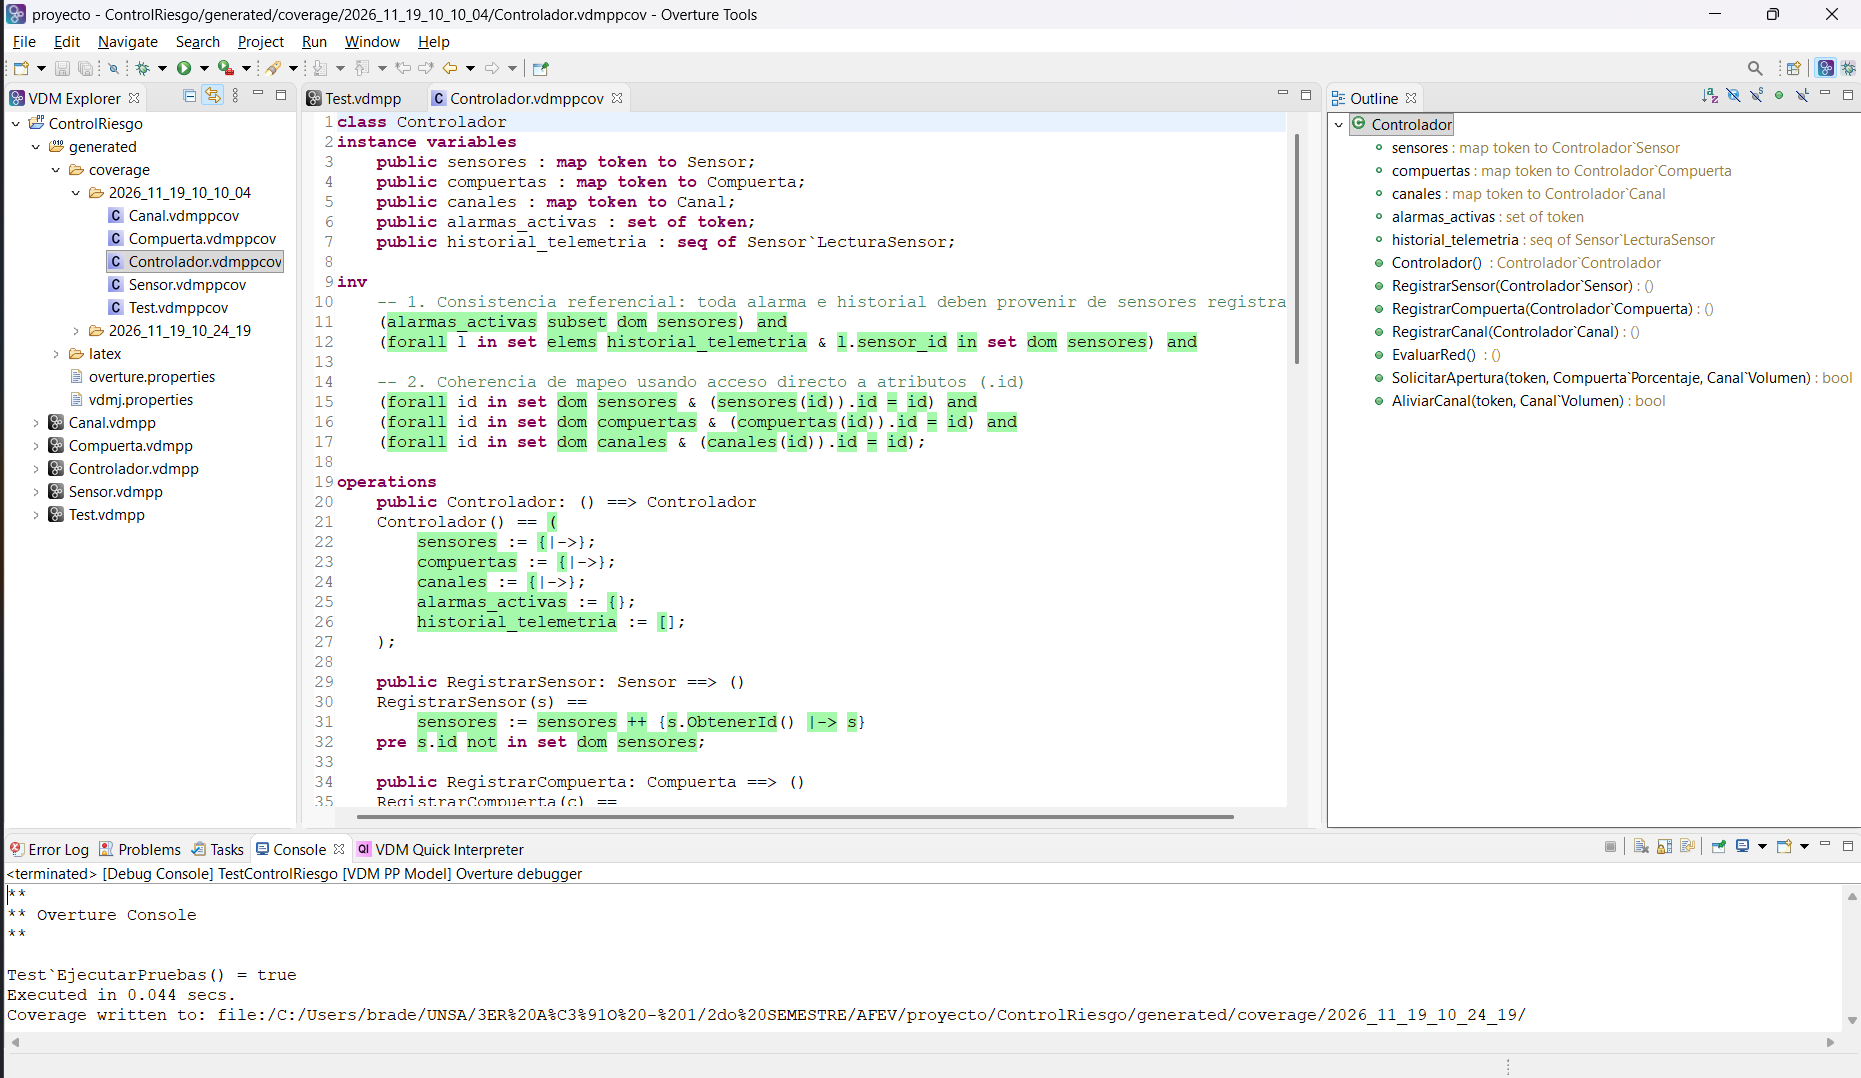
\includegraphics[width=\columnwidth]{fig/cobertura_overture.png}
\caption{Ejecución de \texttt{Test\textasciigrave{}EjecutarPruebas() = true} y cobertura en verde de \texttt{Controlador.vdmppcov} en Overture Tool v3.0.2.}
\label{fig:cobertura_overture}
\end{figure}

\begin{figure}[htbp]
\centering
\begin{tabular}{@{}c@{\hspace{4pt}}c@{}}
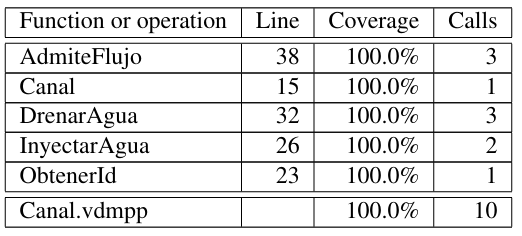
\includegraphics[width=0.48\columnwidth]{fig/cobertura_canal.png} &
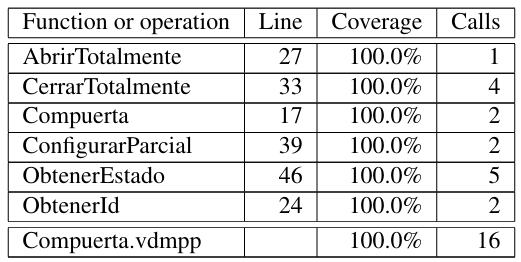
\includegraphics[width=0.48\columnwidth]{fig/cobertura_compuerta.png} \\
{\scriptsize (a) \texttt{Canal.vdmpp} (100.0\%)} & {\scriptsize (b) \texttt{Compuerta.vdmpp} (100.0\%)} \\[6pt]
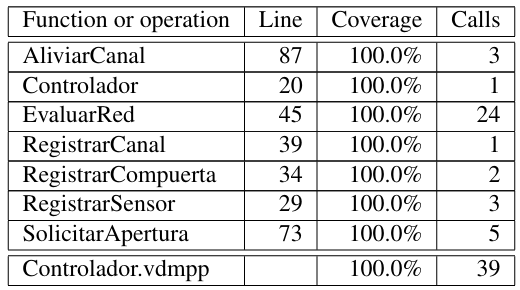
\includegraphics[width=0.48\columnwidth]{fig/cobertura_controlador.png} &
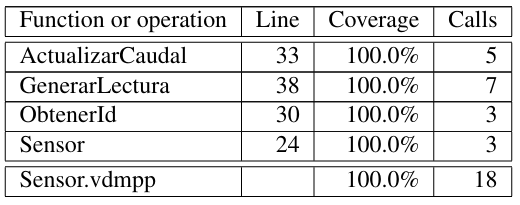
\includegraphics[width=0.48\columnwidth]{fig/cobertura_sensor.png} \\
{\scriptsize (c) \texttt{Controlador.vdmpp} (100.0\%)} & {\scriptsize (d) \texttt{Sensor.vdmpp} (100.0\%)} \\[6pt]
\multicolumn{2}{c}{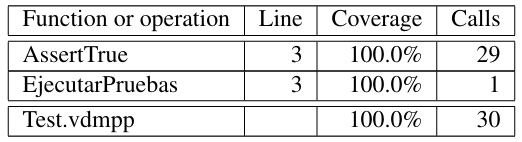
\includegraphics[width=0.52\columnwidth]{fig/cobertura_test.png}} \\
\multicolumn{2}{c}{{\scriptsize (e) \texttt{Test.vdmpp} (100.0\%)}} \\
\end{tabular}
\caption{Reportes individuales de cobertura de pruebas al 100.0\% generados por Overture Tool v3.0.2 para las cinco clases.}
\label{fig:cobertura_tablas}
\end{figure}

\section{Verificación Formal por Model Checking (UPPAAL 5.0)}
Mientras que VDM++ garantiza la solidez estructural de invariantes y contratos de datos, la evaluación de los márgenes reales de reacción ante retardos electromecánicos y frecuencias de muestreo requiere verificación temporizada \cite{behrmann2004tutorial}. Para ello, se construyó una red de autómatas temporizados en \textbf{UPPAAL 5.0.0 (Win64)} basada en la teoría de Alur y Dill \cite{alur1994theory,bengtsson2004timed}.

\subsection{Declaraciones del Sistema, Relojes e Histéresis}
El sistema opera sobre la variable entera acotada $\text{volumen} \in [0, 150]$ (iniciando en $50$), con $\text{MAX\_CAPACIDAD} = 100$, umbral de disparo $\text{NIVEL\_PELIGRO} = 80$ y umbral de histéresis $\text{NIVEL\_SEGURO} = 60$. Se incorporan dos parámetros temporales de actuación física: $T_{\text{CIERRE}}$ (nominal $6\,\text{s}$) y $T_{\text{APERTURA}} = 2\,\text{s}$, junto con seis canales \texttt{broadcast}: \texttt{alerta\_peligro}, \texttt{alerta\_segura}, \texttt{cerrar\_compuerta}, \texttt{abrir\_compuerta}, \texttt{compuerta\_cerrada} y \texttt{compuerta\_abierta} (Fig. \ref{fig:declaraciones}).

\begin{figure}[htbp]
\centering
\begin{tabular}{cc}
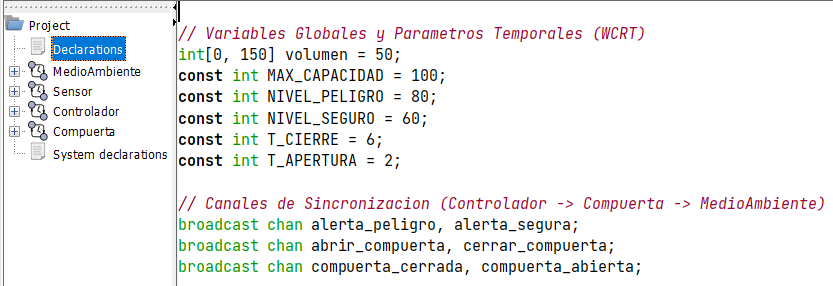
\includegraphics[width=0.45\columnwidth]{fig/declaraciones_globales.png} &
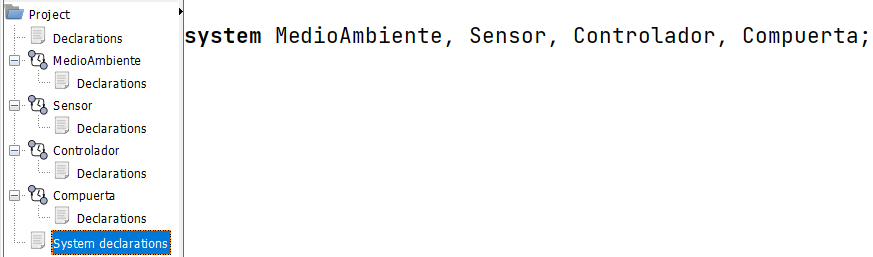
\includegraphics[width=0.45\columnwidth]{fig/declaraciones_sistema.png} \\
{\scriptsize (a) Declaraciones Globales} & {\scriptsize (b) Declaraciones del Sistema} \\[8pt]
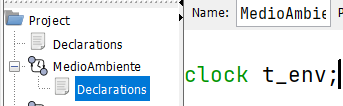
\includegraphics[width=0.45\columnwidth]{fig/declaraciones_ambiente.png} &
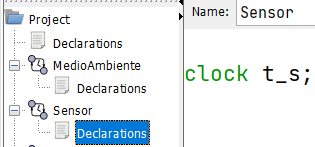
\includegraphics[width=0.45\columnwidth]{fig/declaraciones_sensor.png} \\
{\scriptsize (c) Reloj Local: \texttt{MedioAmbiente}} & {\scriptsize (d) Reloj Local: \texttt{Sensor}} \\
\end{tabular}
\caption{Declaraciones globales, instancias del sistema y relojes locales en UPPAAL.}
\label{fig:declaraciones}
\end{figure}

\subsection{Red de Autómatas Temporizados con Acoplamiento Real}
La red corrige el modelo idealizado de tiempo cero al desacoplar completamente la orden del controlador de la dinámica hidráulica del canal mediante cuatro procesos concurrentes (Fig. \ref{fig:automatas}):
\begin{itemize}
    \item \textbf{Sensor (\texttt{t\_s <= 1}):} Muestrea el volumen cada $1\,\text{s}$. Transita a \texttt{Critico} emitiendo \texttt{alerta\_peligro!} cuando $\text{volumen} \geq 80$, pero implementa histéresis manteniendo la alarma hasta que $\text{volumen} \leq 60$, instante en que emite \texttt{alerta\_segura!} para prevenir oscilaciones destructivas (\textit{chattering}).
    \item \textbf{Controlador:} Utiliza ubicaciones comprometidas (\textit{committed}) en \texttt{ProcesandoPeligro} y \texttt{ProcesandoSeguro} para despachar instantáneamente ($\Delta t = 0$) la orden lógica \texttt{cerrar\_compuerta!} o \texttt{abrir\_compuerta!} hacia el actuador.
    \item \textbf{Compuerta (\texttt{clock t\_act}):} Modela el recorrido electromecánico real mediante los estados intermedios \texttt{Cerrando} ($t_{\text{act}} \leq T_{\text{CIERRE}}$) y \texttt{Abriendo} ($t_{\text{act}} \leq T_{\text{APERTURA}}$). Recién al completar el recorrido emite \texttt{compuerta\_cerrada!} o \texttt{compuerta\_abierta!}.
    \item \textbf{MedioAmbiente (\texttt{t\_env <= 2}):} En \texttt{Llenando} incrementa el volumen en $+5$ cada $2\,\text{s}$ incluso durante \texttt{Compuerta.Cerrando}; solo conmuta a \texttt{Drenando} ($-5$ cada $2\,\text{s}$) cuando recibe \texttt{compuerta\_cerrada?}, incluyendo guarda de saturación superior y bucle de resguardo cuando $\text{volumen} < 5$ para impedir bloqueos temporales.
\end{itemize}

\begin{figure}[htbp]
\centering
\begin{tabular}{cc}
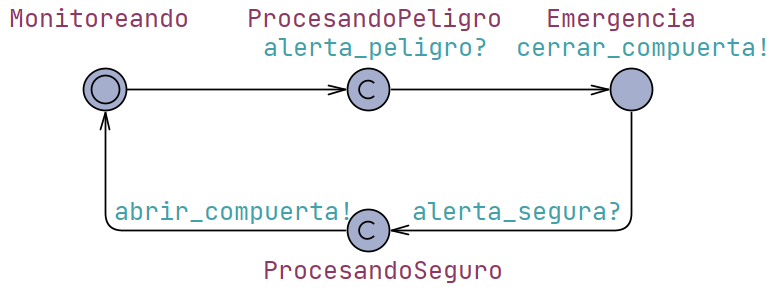
\includegraphics[width=0.45\columnwidth]{fig/automata_controlador.png} &
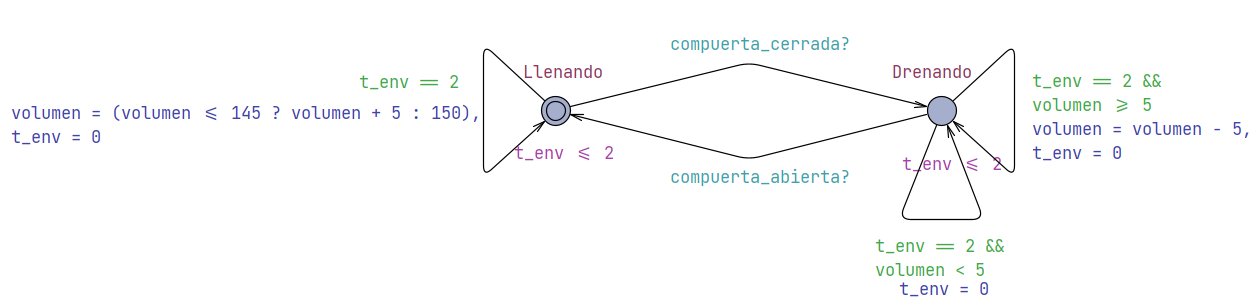
\includegraphics[width=0.45\columnwidth]{fig/automata_ambiente.png} \\
{\scriptsize (a) Autómata \texttt{Controlador}} & {\scriptsize (b) Autómata \texttt{MedioAmbiente}} \\[8pt]
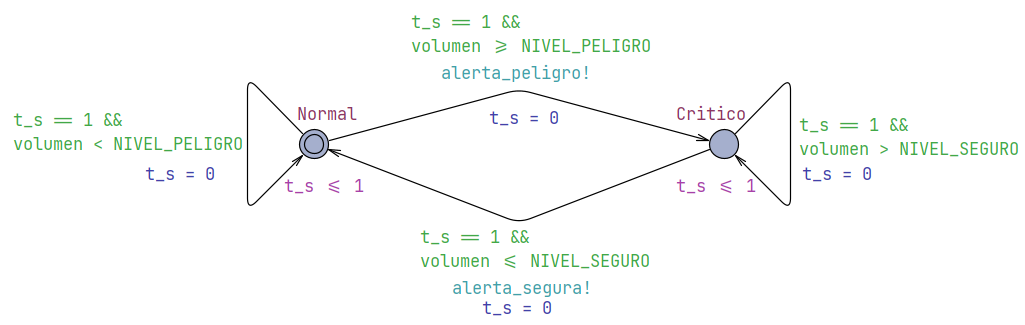
\includegraphics[width=0.45\columnwidth]{fig/automata_sensor.png} &
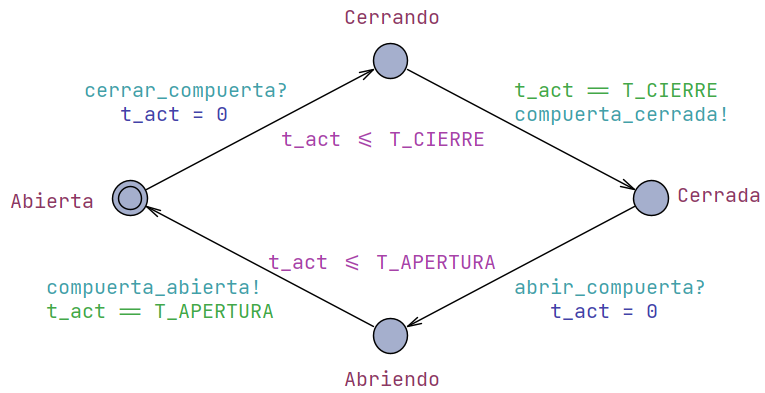
\includegraphics[width=0.45\columnwidth]{fig/automata_compuerta.png} \\
{\scriptsize (c) Autómata \texttt{Sensor}} & {\scriptsize (d) Autómata \texttt{Compuerta}} \\
\end{tabular}
\caption{Red de Autómatas Temporizados en UPPAAL 5.0.}
\label{fig:automatas}
\end{figure}

\subsection{Análisis WCRT: Contraejemplo vs. Cota Certificada}
El análisis formal de fase entre el reloj de muestreo ($T_s = 1\,\text{s}$) y el ritmo de llenado ($T_{\text{env}} = 2\,\text{s}$, $+5\,\text{m}^3$) revela que, en el peor desfase posible, el sensor acaba de muestrear $75\,\text{m}^3$ en el instante en que el canal sube a $80\,\text{m}^3$. Ello introduce un retardo de detección de $1\,\text{s}$ con $t_{\text{env}} = 1$ acumulado. Durante el cierre físico, el quinto incremento (que eleva el volumen a $105\,\text{m}^3 > 100$) ocurre a los $9\,\text{s}$ de iniciada la maniobra. En consecuencia, todo actuador con $T_{\text{CIERRE}} \geq 9\,\text{s}$ viola la seguridad del canal.

Para demostrar este hallazgo mediante \texttt{verifyta.exe}, se evaluó el modelo de contraejemplo \texttt{ControlRiesgo\_Contraejemplo.xml} ($T_{\text{CIERRE}} = 10\,\text{s}$) y se ejecutó un barrido de sensibilidad alrededor de la frontera (Tabla \ref{tab:wcrt}). La traza diagnóstica obtenida para $T_{\text{CIERRE}} = 10\,\text{s}$ confirma que en $t_{\text{act}} = 9\,\text{s}$, mientras la compuerta permanece en \texttt{Cerrando}, el ambiente ejecuta una nueva inyección llevando la variable a $\text{volumen} = 105$ antes de alcanzar \texttt{Compuerta.Cerrada} en $t_{\text{act}} = 10\,\text{s}$. Por el contrario, con $T_{\text{CIERRE}} = 8\,\text{s}$ el volumen toca exactamente $100\,\text{m}^3$, y con el valor nominal $T_{\text{CIERRE}} = 6\,\text{s}$ (\texttt{ControlRiesgo.xml}) el pico máximo verificado es $95\,\text{m}^3$, preservando $5\,\text{m}^3$ de resguardo.

\begin{table}[htbp]
\caption{Barrido de Sensibilidad WCRT en \texttt{verifyta.exe} (UPPAAL 5.0)}
\begin{center}
\resizebox{\columnwidth}{!}{
\begin{tabular}{|c|c|c|c|l|}
\hline
\textbf{$T_{\text{CIERRE}}$ (s)} & \textbf{Pico Máx.} & \textbf{Estado $A[]\,\text{vol} \leq 100$} & \textbf{Margen Libre} & \textbf{Interpretación Formal} \\
\hline
6 & $95\,\text{m}^3$ & \textbf{Satisfecho (Verde)} & $5\,\text{m}^3$ & Operación nominal segura (\texttt{ControlRiesgo.xml}). \\
8 & $100\,\text{m}^3$ & \textbf{Satisfecho (Verde)} & $0\,\text{m}^3$ & Cota límite matemática (supremo admisible). \\
9 & $105\,\text{m}^3$ & \textbf{Falla (Rojo)} & $-5\,\text{m}^3$ & Violación exacta en frontera de entrelazado. \\
10 & $105\,\text{m}^3$ & \textbf{Falla (Rojo)} & $-5\,\text{m}^3$ & Contraejemplo formal (\texttt{ControlRiesgo\_Contraejemplo.xml}). \\
\hline
\end{tabular}
}
\label{tab:wcrt}
\end{center}
\end{table}

\subsection{Simulación Concreta y Verificación CTL}
La Fig. \ref{fig:simulador} representa la dinámica esperada en el simulador concreto donde el volumen rebasa el umbral de $80\,\text{m}^3$ mientras transcurre el cierre físico, invierte su pendiente al completarse la señal \texttt{compuerta\_cerrada!} y desciende de manera continua hasta cruzar la histéresis de $60\,\text{m}^3$. En la Tabla \ref{tab:ctl} y la Fig. \ref{fig:verifier} se resumen las 7 propiedades CTL verificadas con resultado favorable en \texttt{ControlRiesgo.xml} ($T_{\text{CIERRE}} = 6\,\text{s}$).

\begin{figure}[htbp]
\centering
\begin{tabular}{@{}c@{\hspace{4pt}}c@{}}
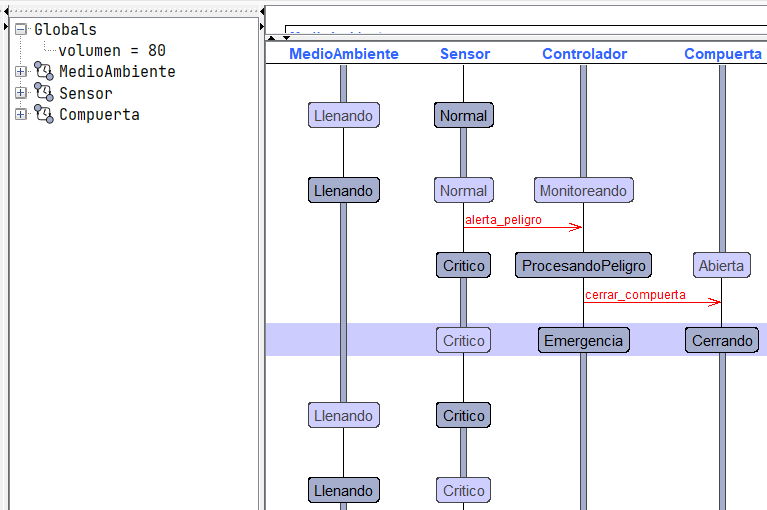
\includegraphics[width=0.48\columnwidth]{fig/simulacion_inicio_cierre.png} &
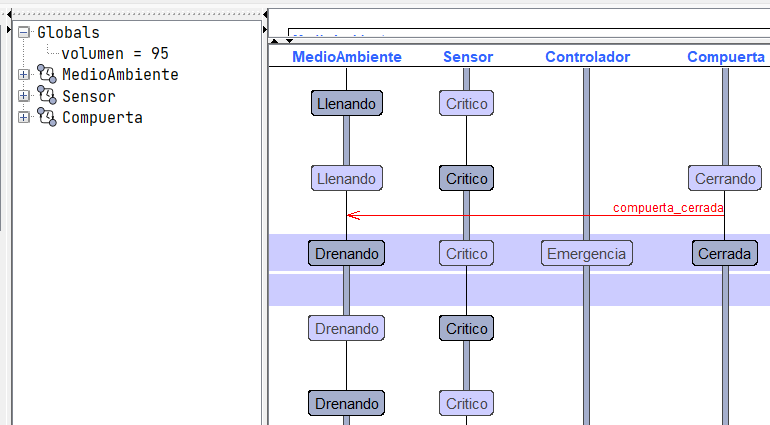
\includegraphics[width=0.48\columnwidth]{fig/simulacion_volumen.png} \\
{\scriptsize (a) Disparo ($\text{vol}=80$, \texttt{Cerrando})} & {\scriptsize (b) Cierre ($\text{vol}=95$, \texttt{Drenando})} \\[6pt]
\multicolumn{2}{c}{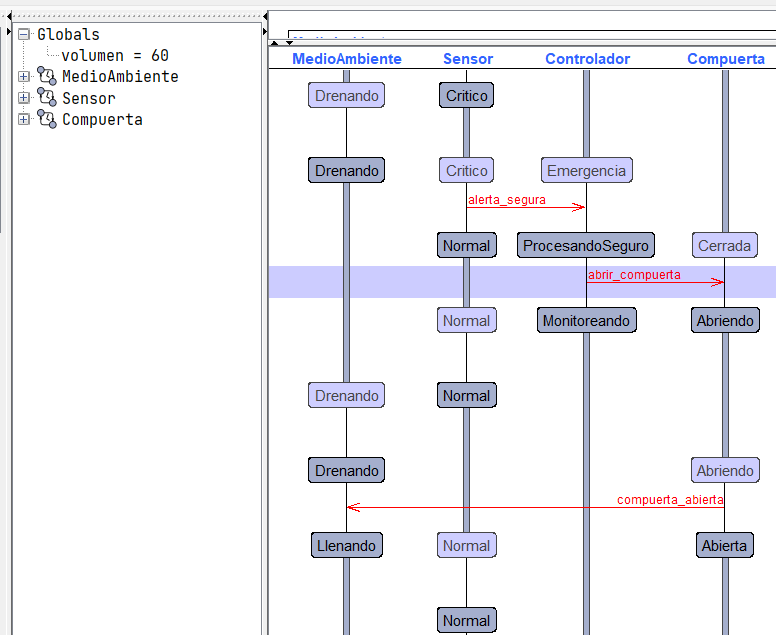
\includegraphics[width=0.72\columnwidth]{fig/simulacion_recuperacion.png}} \\
\multicolumn{2}{c}{{\scriptsize (c) Recuperación por histéresis ($\text{vol}=60$, \texttt{Abriendo} $\rightarrow$ \texttt{Abierta})}} \\
\end{tabular}
\caption{Traza de simulación concreta en UPPAAL: (a) inicio de cierre mientras continúa el llenado, (b) pico contenido en $95\,\text{m}^3$ al emitirse \texttt{compuerta\_cerrada} y (c) reapertura controlada en $60\,\text{m}^3$.}
\label{fig:simulador}
\end{figure}

\begin{table}[htbp]
\caption{Evaluación Formal de Propiedades CTL en UPPAAL ($T_{\text{CIERRE}} = 6\,\text{s}$)}
\begin{center}
\resizebox{\columnwidth}{!}{
\begin{tabular}{|c|l|p{4.3cm}|}
\hline
\textbf{\#} & \textbf{Fórmula CTL} & \textbf{Demostración Matemática} \\
\hline
1 & \texttt{A[] not deadlock} & \textit{Deadlock-freedom:} Ausencia absoluta de bloqueos en cualquier entrelazado. Cumple RNF2. \\
\hline
2 & \texttt{A[] volumen <= MAX\_CAPACIDAD} & \textit{Safety WCRT:} Garantiza contención ($\leq 95 \leq 100$) bajo la cota $T_{\text{CIERRE}} \leq 8\,\text{s}$. Cumple RNF1. \\
\hline
3 & \texttt{E<> Controlador.Emergencia} & \textit{Reachability:} El estado de emergencia es alcanzable. \\
\hline
4 & \texttt{Sensor.Critico --> Compuerta.Cerrada} & \textit{Liveness:} Toda detección crítica conduce al cierre físico completo tras $T_{\text{CIERRE}}$. \\
\hline
5 & \texttt{E<> MedioAmbiente.Drenando} & \textit{Reachability:} El drenaje físico del canal se activa solo tras confirmarse el cierre. Cumple RF6. \\
\hline
6 & \texttt{A[] (Compuerta.Abierta imply MedioAmbiente.Llenando)} & \textit{Coherencia:} Invariante física que prohíbe estados desfasados entre actuador y canal. \\
\hline
7 & \texttt{Sensor.Critico --> (Controlador.Monitoreando and volumen <= 60)} & \textit{Histéresis:} Garantiza retorno estable tras drenar hasta \texttt{NIVEL\_SEGURO = 60} sin \textit{chattering}. \\
\hline
\end{tabular}
}
\label{tab:ctl}
\end{center}
\end{table}

\begin{figure}[htbp]
\centering
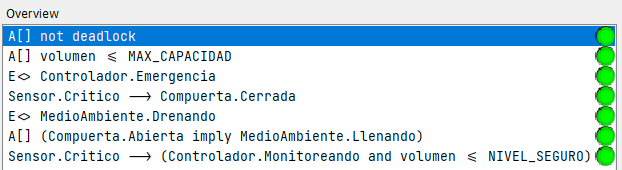
\includegraphics[width=\columnwidth]{fig/verificacion_propiedades.png}
\vspace{4pt}
{\scriptsize (a) Modelo certificado \texttt{ControlRiesgo.xml} ($T_{\text{CIERRE}}=6\,\text{s}$): 7/7 propiedades en verde.} \\[6pt]
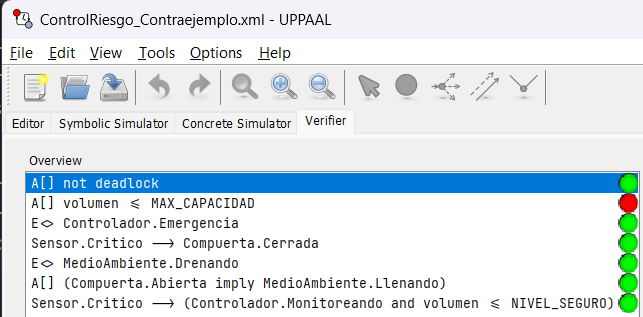
\includegraphics[width=\columnwidth]{fig/contraejemplo_desborde.png}
\vspace{2pt}
{\scriptsize (b) Contraejemplo \texttt{ControlRiesgo\_Contraejemplo.xml} ($T_{\text{CIERRE}}=10\,\text{s}$): falla en rojo.}
\caption{Evidencia comparativa en el Verifier de UPPAAL 5.0: (a) certificación dentro de la cota WCRT y (b) violación de seguridad por cierre lento.}
\label{fig:verifier}
\end{figure}

\subsection{Extensión Tolerante a Fallos Mecánicos (\textit{Watchdog} y Aliviadero)}
Para cubrir fallos físicos del actuador por sedimentos u obstrucciones, se modeló de forma independiente la variante \texttt{ControlRiesgo\_ToleranteFallos.xml} incorporando un quinto autómata \texttt{Aliviadero} ($T_{\text{alivio}} = 2\,\text{s}$), una transición no determinista desde \texttt{Compuerta.Cerrando} hacia \texttt{Compuerta.Atascada} ($T_{\text{cierre}} = 4\,\text{s}$) y un temporizador \textit{Watchdog} ($T_{\text{watchdog}} = 5\,\text{s}$) en \texttt{Controlador.EsperandoCierre}. Si el cierre físico no se confirma antes de expirar el \textit{Watchdog}, el controlador activa \texttt{activar\_aliviadero!} y transita a \texttt{ModoFalloSeguro} sin intentar reabrir la compuerta averiada. La verificación exhaustiva en \texttt{verifyta.exe} confirmó satisfacción total ($6/6$ fórmulas) en \texttt{ControlRiesgo\_ToleranteFallos.q} (Fig. \ref{fig:tolerante_fallos}): ausencia de bloqueos (\texttt{A[] not deadlock}), contención garantizada aun bajo atasco (\texttt{A[] volumen <= MAX\_CAPACIDAD}), alcanzabilidad de \texttt{Compuerta.Atascada} y \texttt{Aliviadero.Abierto}, vivacidad alternativa (\texttt{Sensor.Critico --> (Compuerta.Cerrada or Aliviadero.Abierto)}) y coherencia (\texttt{A[] (Controlador.ModoFalloSeguro imply Compuerta.Atascada)}).

\begin{figure}[htbp]
\centering
\begin{tabular}{@{}c@{\hspace{4pt}}c@{}}
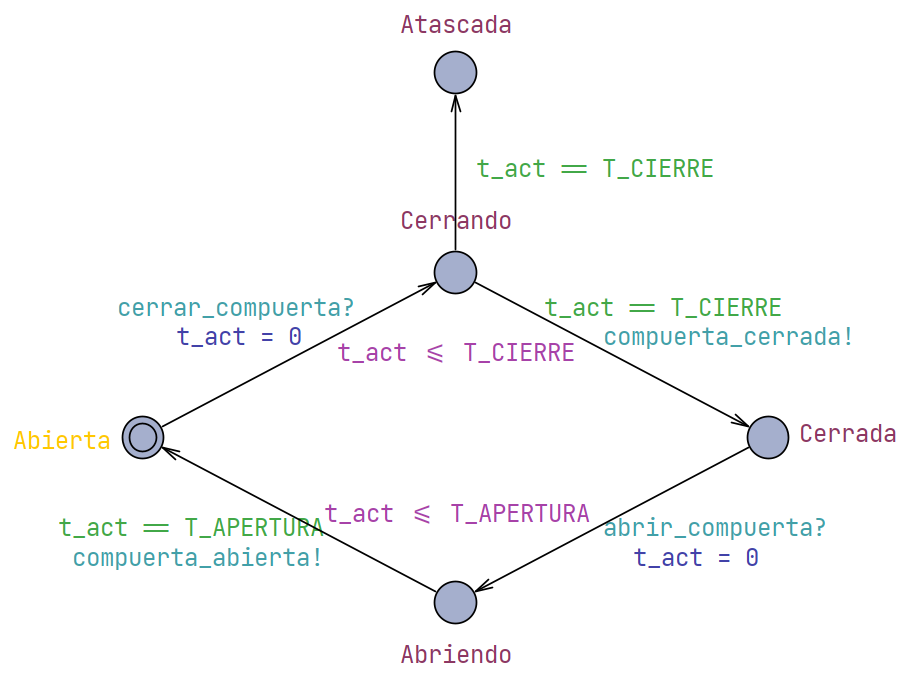
\includegraphics[width=0.48\columnwidth]{fig/automata_compuerta_fallos.png} &
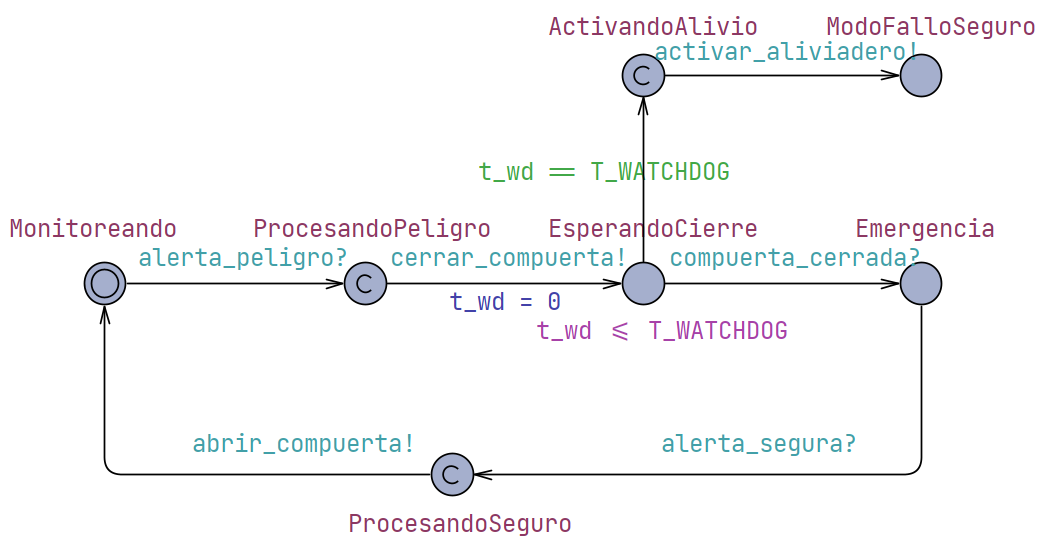
\includegraphics[width=0.48\columnwidth]{fig/automata_controlador_fallos.png} \\
{\scriptsize (a) \texttt{Compuerta} con estado \texttt{Atascada}.} &
{\scriptsize (b) \texttt{Controlador} con \textit{Watchdog}.} \\[4pt]
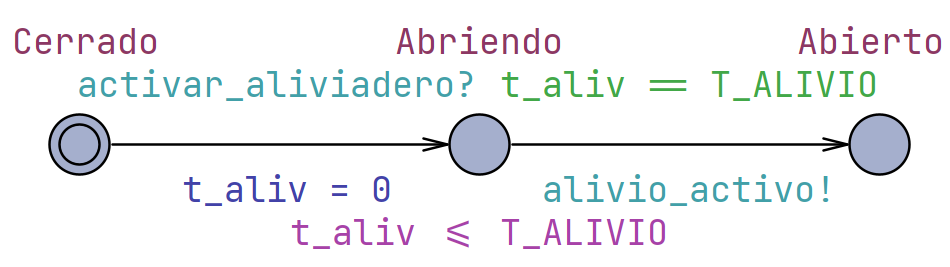
\includegraphics[width=0.48\columnwidth]{fig/automata_aliviadero.png} &
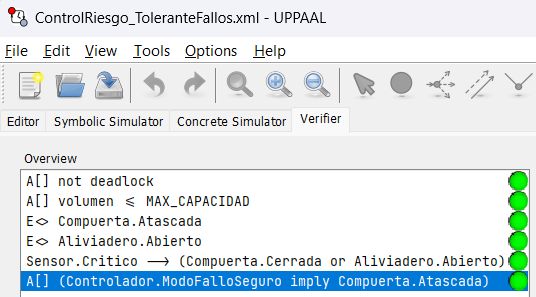
\includegraphics[width=0.48\columnwidth]{fig/verificacion_tolerante_fallos.png} \\
{\scriptsize (c) \texttt{Aliviadero} ($T_{\text{ALIVIO}}=2\,\text{s}$).} &
{\scriptsize (d) Verificación CTL ($6/6$ en verde).}
\end{tabular}
\caption{Extensión tolerante a fallos en UPPAAL 5.0: (a) compuerta con atasco, (b) controlador con \textit{Watchdog}, (c) aliviadero y (d) verificación CTL completa.}
\label{fig:tolerante_fallos}
\end{figure}

\section{Discusión de Resultados}
La articulación entre VDM++ y UPPAAL evidencia por qué un SCADA agrícola tradicional no puede certificar seguridad por sí solo:
\begin{itemize}
    \item \textbf{Control preventivo gradual y trazabilidad en VDM++:} La inclusión de estrangulamiento parcial al $50\%$ en \texttt{<PRECAUCION>}, el balance directo de volumen sobre \texttt{Canal} desde el \texttt{Controlador} y el registro secuencial \texttt{historial\_telemetria} eliminan brechas entre la especificación de datos y la operación de red.
    \item \textbf{Cuantificación WCRT frente a heurísticas de PLC:} Un PLC programado con umbrales arbitrarios asume cierres instantáneos; el contraejemplo obtenido en UPPAAL demuestra que si la compuerta mecánica tarda $9\,\text{s}$ o más en cerrar, el desborde a $105\,\text{m}^3$ es inevitable. Determinar la cota $T_{\text{cierre}} \leq 8\,\text{s}$ e imponer la banda de histéresis $[60, 80]\,\text{m}^3$ provee criterios cuantitativos de diseño mecánico y eléctrico antes de desplegar hardware en campo.
\end{itemize}

\section{Conclusiones y Trabajo Futuro}
En este trabajo se reformuló el diseño y verificación formal de un sistema SCADA para compuertas de riego, trascendiendo un control binario idealizado hacia un marco formal de verificación de márgenes temporales de reacción (WCRT) y control preventivo en tres niveles. En VDM++, se unificó la especificación orientada a objetos con invariantes completos sobre \texttt{LecturaSensor}, coherencia por acceso directo a atributos, gestión conjunta de \texttt{Set}, \texttt{Seq} y \texttt{Map} y validación limpia en Overture v3.0.2. En UPPAAL 5.0, el modelado del cierre electromecánico real (\texttt{Cerrando}) e histéresis demostró mediante contraejemplo la falla por desbordamiento para $T_{\text{cierre}} \geq 9\,\text{s}$ y certificó matemáticamente las siete propiedades CTL dentro de la frontera $T_{\text{cierre}} \leq 8\,\text{s}$ (pico de $95\,\text{m}^3$ en operación nominal a $6\,\text{s}$).

Como trabajo futuro se proyecta la traducción de las reglas certificadas hacia lógica de autómatas industriales mediante \textit{PLCverif} \cite{lopezmiguel2021plcverif} y el acoplamiento hidrodinámico de múltiples tramos en cascada.

\section*{Anexos: Enlaces del Proyecto}
Artefactos digitales y repositorio oficial del proyecto:
\begin{itemize}
    \item \textbf{Repositorio en GitHub (Código Fuente VDM++ y Modelos UPPAAL):} \\
    \href{https://github.com/DenilsonCB/verificacion-formal-compuertas-agricolas-vdmpp-uppaal}{\texttt{https://github.com/DenilsonCB/\allowbreak verificacion-formal-\allowbreak compuertas-agricolas-\allowbreak vdmpp-uppaal}} \\
    \textit{Contiene la carpeta \texttt{ControlRiesgo/}, los modelos de \texttt{UPPAAL/} (\texttt{ControlRiesgo.xml}, \texttt{ControlRiesgo\_Contraejemplo.xml}, \texttt{ControlRiesgo\_ToleranteFallos.xml}, archivos \texttt{.q}), el artículo LaTeX y las diapositivas.}
    \item \textbf{Diapositivas de Exposición:} \\
    \texttt{exposicion\_\allowbreak final\_\allowbreak proyecto/\allowbreak diapositivas\_\allowbreak finales.pdf} \\
    \textit{Material de sustentación compilado en Typst e integrado en el documento unificado \texttt{articulo\_\allowbreak y\_\allowbreak diapositivas\_\allowbreak unificado.pdf}.}
\end{itemize}

\bibliographystyle{IEEEtran}
\bibliography{refs}

\end{document}
